\documentclass{beamer}
\usepackage{tikz}
\usetikzlibrary{arrows.meta, decorations.pathreplacing, calc}

% ------------------------------------------------------------------
% Theme colors & styles: blkline / blkfill / accentline / accentfill /
% lbl / flow. Assumed to already exist in your master preamble — delete
% this block if dropping these frames into that file.
% ------------------------------------------------------------------
\definecolor{blkline}{HTML}{375775}
\definecolor{blkfill}{HTML}{EAF0F7}
\definecolor{accentline}{HTML}{B5651D}
\definecolor{accentfill}{HTML}{FBEEDD}
\tikzset{
  lbl/.style={text=black},
  flow/.style={-{Stealth[length=2.2mm]}, thick},
  loadedbox/.style={draw=blkline, fill=blkfill, thick},      % register byte actually stored
  extbox/.style={draw=blkline, fill=blkfill!35, thick, dashed},   % register byte not used
  memwrite/.style={draw=accentline, fill=accentfill, thick},      % memory byte overwritten
  memkeep/.style={draw=accentline, fill=accentfill!35, thick, dashed}, % memory byte unchanged
}

% shared geometry
\def\bw{1.0}
\def\rh{0.62}
\def\regx{0.7}
\def\regy{4.3}
\def\memx{5.2}
\def\memy{3.0}

\begin{document}

% ==================================================================
% STR — store a full word
% ==================================================================
\begin{frame}{STR: Storing a Word to Memory}
\centering
{\small\itshape Before: R1 = 0x11223344, \quad [0x40020014] = 0x00C0FFEE\par}
\vspace{2mm}
\resizebox{0.92\textwidth}{!}{%
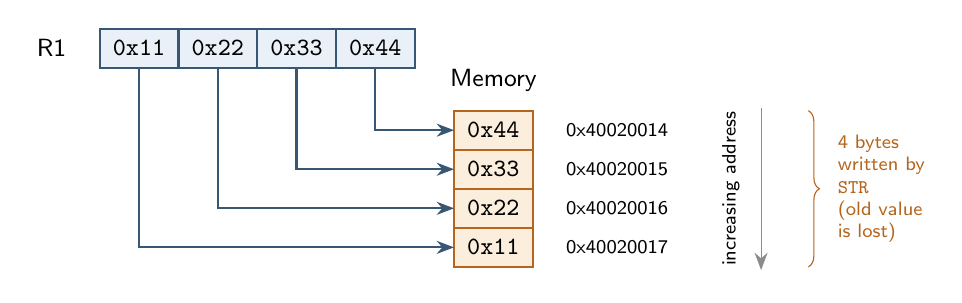
\begin{tikzpicture}[x=10mm, y=8mm]

% --- Register R1: all four bytes are stored ---
\foreach \p/\val in {0/{0x11}, 1/{0x22}, 2/{0x33}, 3/{0x44}}{
  \pgfmathsetmacro{\x}{\regx+\p*\bw}
  \draw[loadedbox] (\x,\regy) rectangle ({\x+\bw},{\regy-\rh});
  \node[font=\ttfamily\small] at ({\x+\bw/2},{\regy-\rh/2}) {\val};
}
\node[lbl, anchor=east, font=\sffamily\small] at ({\regx-0.3},{\regy-\rh/2}) {R1};

% --- Memory: all four bytes overwritten, low address on top (LSB) ---
\foreach \i/\val/\addr in {%
    0/{0x44}/{0x40020014},
    1/{0x33}/{0x40020015},
    2/{0x22}/{0x40020016},
    3/{0x11}/{0x40020017}}{
  \pgfmathsetmacro{\y}{\memy-\i*\rh}
  \draw[memwrite] (\memx,\y) rectangle ({\memx+\bw},{\y-\rh});
  \node[font=\ttfamily\small] at ({\memx+\bw/2},{\y-\rh/2}) {\val};
  \node[lbl, anchor=west, font=\sffamily\scriptsize] at ({\memx+\bw+0.3},{\y-\rh/2}) {\addr};
}
\node[lbl, anchor=south, font=\sffamily\small] at ({\memx+\bw/2},{\memy+0.15}) {Memory};

% --- Arrows: all four bytes flow down from register into memory ---
\draw[flow, draw=blkline] ({\regx+3*\bw+\bw/2},{\regy-\rh}) |- (\memx,{\memy-0*\rh-\rh/2});
\draw[flow, draw=blkline] ({\regx+2*\bw+\bw/2},{\regy-\rh}) |- (\memx,{\memy-1*\rh-\rh/2});
\draw[flow, draw=blkline] ({\regx+1*\bw+\bw/2},{\regy-\rh}) |- (\memx,{\memy-2*\rh-\rh/2});
\draw[flow, draw=blkline] ({\regx+0*\bw+\bw/2},{\regy-\rh}) |- (\memx,{\memy-3*\rh-\rh/2});

% --- Address axis + brace ---
\def\axisx{9.1}
\draw[-{Stealth[length=2.2mm]}, draw=black!45]
    ({\axisx},{\memy+0.05}) -- ({\axisx},{\memy-4*\rh-0.05});
\node[lbl, anchor=south, rotate=90, font=\sffamily\scriptsize]
    at ({\axisx-0.15},{\memy-2*\rh}) {increasing address};
\draw[decorate, decoration={brace, amplitude=4pt}, draw=accentline]
    ({\axisx+0.6},{\memy}) -- ({\axisx+0.6},{\memy-4*\rh});
\node[lbl, anchor=west, align=left, font=\sffamily\scriptsize, text=accentline]
    at ({\axisx+0.85},{\memy-2*\rh}) {4 bytes\\written by\\\texttt{STR}\\(old value\\is lost)};

\end{tikzpicture}%
}
\end{frame}

% ==================================================================
% STRH — store the low halfword only
% ==================================================================
\begin{frame}{STRH: Storing a Halfword to Memory}
\centering
{\small\itshape Before: R1 = 0x11223344, \quad [0x40020014] = 0x00C0FFEE\par}
\vspace{2mm}
\resizebox{0.92\textwidth}{!}{%
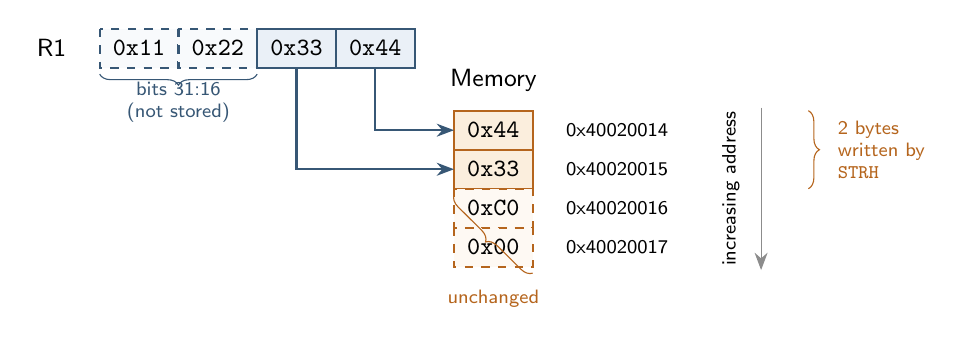
\begin{tikzpicture}[x=10mm, y=8mm]

% --- Register R1: only byte1,byte0 (low halfword) are stored ---
\foreach \p/\val/\used in {0/{0x11}/0, 1/{0x22}/0, 2/{0x33}/1, 3/{0x44}/1}{
  \pgfmathsetmacro{\x}{\regx+\p*\bw}
  \ifnum\used=1
    \draw[loadedbox] (\x,\regy) rectangle ({\x+\bw},{\regy-\rh});
  \else
    \draw[extbox] (\x,\regy) rectangle ({\x+\bw},{\regy-\rh});
  \fi
  \node[font=\ttfamily\small] at ({\x+\bw/2},{\regy-\rh/2}) {\val};
}
\node[lbl, anchor=east, font=\sffamily\small] at ({\regx-0.3},{\regy-\rh/2}) {R1};

% under-brace: high halfword not stored
\draw[decorate, decoration={brace, amplitude=4pt, mirror}, draw=blkline]
    ({\regx},{\regy-\rh-0.1}) -- ({\regx+2*\bw},{\regy-\rh-0.1});
\node[lbl, font=\sffamily\scriptsize, text=blkline, align=center]
    at ({\regx+\bw},{\regy-\rh-0.55}) {bits 31:16\\(not stored)};

% --- Memory: low 2 bytes overwritten, high 2 bytes keep their old value ---
\foreach \i/\val/\addr/\written in {%
    0/{0x44}/{0x40020014}/1,
    1/{0x33}/{0x40020015}/1,
    2/{0xC0}/{0x40020016}/0,
    3/{0x00}/{0x40020017}/0}{
  \pgfmathsetmacro{\y}{\memy-\i*\rh}
  \ifnum\written=1
    \draw[memwrite] (\memx,\y) rectangle ({\memx+\bw},{\y-\rh});
  \else
    \draw[memkeep] (\memx,\y) rectangle ({\memx+\bw},{\y-\rh});
  \fi
  \node[font=\ttfamily\small] at ({\memx+\bw/2},{\y-\rh/2}) {\val};
  \node[lbl, anchor=west, font=\sffamily\scriptsize] at ({\memx+\bw+0.3},{\y-\rh/2}) {\addr};
}
\node[lbl, anchor=south, font=\sffamily\small] at ({\memx+\bw/2},{\memy+0.15}) {Memory};

% under-brace: unchanged memory bytes
\draw[decorate, decoration={brace, amplitude=4pt, mirror}, draw=accentline]
    ({\memx},{\memy-2*\rh-0.1}) -- ({\memx+\bw},{\memy-4*\rh-0.1});
\node[lbl, font=\sffamily\scriptsize, text=accentline, align=center]
    at ({\memx+\bw/2},{\memy-4*\rh-0.5}) {unchanged};

% --- Arrows: 2 bytes flow down from register into memory ---
\draw[flow, draw=blkline] ({\regx+3*\bw+\bw/2},{\regy-\rh}) |- (\memx,{\memy-0*\rh-\rh/2});
\draw[flow, draw=blkline] ({\regx+2*\bw+\bw/2},{\regy-\rh}) |- (\memx,{\memy-1*\rh-\rh/2});

% --- Address axis + brace ---
\def\axisx{9.1}
\draw[-{Stealth[length=2.2mm]}, draw=black!45]
    ({\axisx},{\memy+0.05}) -- ({\axisx},{\memy-4*\rh-0.05});
\node[lbl, anchor=south, rotate=90, font=\sffamily\scriptsize]
    at ({\axisx-0.15},{\memy-2*\rh}) {increasing address};
\draw[decorate, decoration={brace, amplitude=4pt}, draw=accentline]
    ({\axisx+0.6},{\memy}) -- ({\axisx+0.6},{\memy-2*\rh});
\node[lbl, anchor=west, align=left, font=\sffamily\scriptsize, text=accentline]
    at ({\axisx+0.85},{\memy-1*\rh}) {2 bytes\\written by\\\texttt{STRH}};

\end{tikzpicture}%
}
\end{frame}

% ==================================================================
% STRB — store a single byte
% ==================================================================
\begin{frame}{STRB: Storing a Byte to Memory}
\centering
{\small\itshape Before: R1 = 0x11223344, \quad [0x40020014] = 0x00C0FFEE\par}
\vspace{2mm}
\resizebox{0.92\textwidth}{!}{%
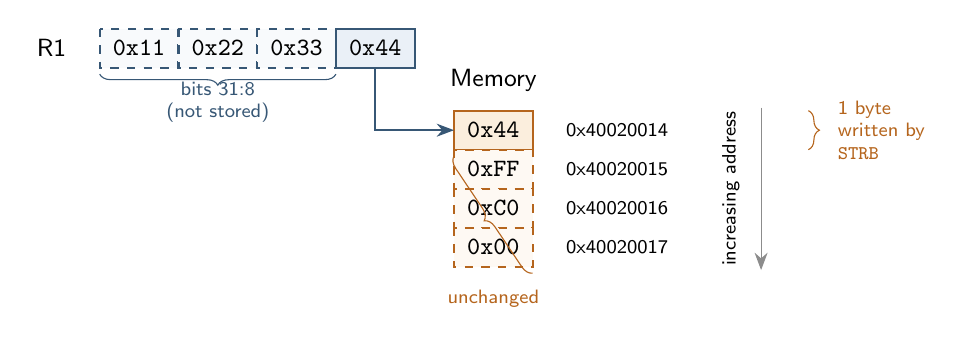
\begin{tikzpicture}[x=10mm, y=8mm]

% --- Register R1: only byte0 (low byte) is stored ---
\foreach \p/\val/\used in {0/{0x11}/0, 1/{0x22}/0, 2/{0x33}/0, 3/{0x44}/1}{
  \pgfmathsetmacro{\x}{\regx+\p*\bw}
  \ifnum\used=1
    \draw[loadedbox] (\x,\regy) rectangle ({\x+\bw},{\regy-\rh});
  \else
    \draw[extbox] (\x,\regy) rectangle ({\x+\bw},{\regy-\rh});
  \fi
  \node[font=\ttfamily\small] at ({\x+\bw/2},{\regy-\rh/2}) {\val};
}
\node[lbl, anchor=east, font=\sffamily\small] at ({\regx-0.3},{\regy-\rh/2}) {R1};

% under-brace: upper 3 bytes not stored
\draw[decorate, decoration={brace, amplitude=4pt, mirror}, draw=blkline]
    ({\regx},{\regy-\rh-0.1}) -- ({\regx+3*\bw},{\regy-\rh-0.1});
\node[lbl, font=\sffamily\scriptsize, text=blkline, align=center]
    at ({\regx+1.5*\bw},{\regy-\rh-0.55}) {bits 31:8\\(not stored)};

% --- Memory: only the low byte overwritten, others keep their old value ---
\foreach \i/\val/\addr/\written in {%
    0/{0x44}/{0x40020014}/1,
    1/{0xFF}/{0x40020015}/0,
    2/{0xC0}/{0x40020016}/0,
    3/{0x00}/{0x40020017}/0}{
  \pgfmathsetmacro{\y}{\memy-\i*\rh}
  \ifnum\written=1
    \draw[memwrite] (\memx,\y) rectangle ({\memx+\bw},{\y-\rh});
  \else
    \draw[memkeep] (\memx,\y) rectangle ({\memx+\bw},{\y-\rh});
  \fi
  \node[font=\ttfamily\small] at ({\memx+\bw/2},{\y-\rh/2}) {\val};
  \node[lbl, anchor=west, font=\sffamily\scriptsize] at ({\memx+\bw+0.3},{\y-\rh/2}) {\addr};
}
\node[lbl, anchor=south, font=\sffamily\small] at ({\memx+\bw/2},{\memy+0.15}) {Memory};

% under-brace: unchanged memory bytes
\draw[decorate, decoration={brace, amplitude=4pt, mirror}, draw=accentline]
    ({\memx},{\memy-1*\rh-0.1}) -- ({\memx+\bw},{\memy-4*\rh-0.1});
\node[lbl, font=\sffamily\scriptsize, text=accentline, align=center]
    at ({\memx+\bw/2},{\memy-4*\rh-0.5}) {unchanged};

% --- Arrow: 1 byte flows down from register into memory ---
\draw[flow, draw=blkline] ({\regx+3*\bw+\bw/2},{\regy-\rh}) |- (\memx,{\memy-0*\rh-\rh/2});

% --- Address axis + brace ---
\def\axisx{9.1}
\draw[-{Stealth[length=2.2mm]}, draw=black!45]
    ({\axisx},{\memy+0.05}) -- ({\axisx},{\memy-4*\rh-0.05});
\node[lbl, anchor=south, rotate=90, font=\sffamily\scriptsize]
    at ({\axisx-0.15},{\memy-2*\rh}) {increasing address};
\draw[decorate, decoration={brace, amplitude=4pt}, draw=accentline]
    ({\axisx+0.6},{\memy}) -- ({\axisx+0.6},{\memy-1*\rh});
\node[lbl, anchor=west, align=left, font=\sffamily\scriptsize, text=accentline]
    at ({\axisx+0.85},{\memy-0.5*\rh}) {1 byte\\written by\\\texttt{STRB}};

\end{tikzpicture}%
}
\end{frame}

\end{document}
